\documentclass{beamer}
%
% Choose how your presentation looks.
%
% For more themes, color themes and font themes, see:
% http://deic.uab.es/~iblanes/beamer_gallery/index_by_theme.html
%
\mode<presentation>
{
  \usetheme{NYU}      % or try Darmstadt, Madrid, Warsaw, ...
  \usecolortheme{default} % or try albatross, beaver, crane, ...
  \usefonttheme{default}  % or try serif, structurebold, ...
  \setbeamertemplate{navigation symbols}{}
  \setbeamertemplate{caption}[numbered]
} 

\usepackage[english]{babel}
\usepackage[utf8x]{inputenc}
\usepackage{multicol}

\title[Big Mortgage Data]{Fair Lending Finder}
\author{Cody Gilbert, Fang Hang, Jeremy Lao}
\institute{NYU Courant, Computer Science}
\date{August 8, 2019}
\titlegraphic{\hfill
\includegraphics[height=1.5cm]{nyu_stacked_color}}

\begin{document}

\begin{frame}
  \titlepage
\end{frame}

% Uncomment these lines for an automatically generated outline.
%\begin{frame}{Outline}
%  \tableofcontents
%\end{frame}

\section{Introduction}

\begin{frame}{Introduction}

\begin{itemize}
  \item How would you like to know your chances of obtaining a mortgage related loan? 
  \item We leverage Home Mortgage Disclosure Act (HMDA) data to tell you just that
\end{itemize}

\vskip 0.5cm

\begin{block}{Example}
Give your application your details and it will return the lender with the highest approval probability: income, loan amount, race, gender, and state
\end{block}

\end{frame}

\section{BDAD Summer 2019}

\subsection{The How}

\begin{frame}{How do we predict? Machine learning, duh}

\begin{eqnarray*}
P(y=k) & = & \ \beta_0 loanAmt_{obs}  \\
& &  + \beta_1 applicantIncome_{obs} \\
& & + \delta_0 race  \\ 
& &  + \delta_1 gender \\
& & +  \delta_2 lender + \epsilon
\end{eqnarray*}

% Commands to include a figure:
%\begin{figure}
%\includegraphics[width=\textwidth]{your-figure's-file-name}
%\caption{\label{fig:your-figure}Caption goes here.}
%\end{figure}

Where $\delta$ are dummy variables for the categorical variables and $\beta$ are coefficients. The outcome (k), approve or deny, $k \in 0,1$

\end{frame}

\subsection{HMDA}

\begin{frame}{Hmm, what is HMDA?}

\begin{itemize}
    \item Home Mortgage Disclosure Act
    \item Lenders are required to collect and report information about housing-related loans to the Consumer Financial Protection Bureau (CFPB)
    \item Data are shared in an anonnymised manner
    \item The CFPB and FDIC both monitor the data to ensure community reinvestment and fair lending
\end{itemize}

\begin{block}{Our Application}
We want to use the data to help you find the lender that will originate your loan
\end{block}


\end{frame}


\section{Infrastructure}
\subsection{Data Sets}
\begin{frame}{Data Sets}

\textbf{Three Data Sets}
\begin{itemize}
    \item Each data set supports and complements the other through offering data that helps provide more information for the analytic
\end{itemize}
\vspace{5mm}
HMDA Data Set \hspace{12mm}  Geo Data \hspace{18mm}  Panel Data
    \begin{multicols}{3}
    \begin{itemize}
        \item $> 125 \ GB$
        \item 2007-2017
        \item Geospatial
        \item $>$50 MB
        \item Reporters
        \item $>$200 MB
    \end{itemize}
    \end{multicols}
\end{frame}

\subsection{Packages}

\begin{frame}{Environments and Tools Used}

\begin{itemize}
    \item Scala Spark \& Maven
    \item Packages: MLLib, Spark Context-RDD, Spark SQL-Dataframes, GeoSpark
    \item Python Plotly
\end{itemize}
\end{frame}

\end{document}

\subsection{Application}

\begin{frame}{Design Diagram}

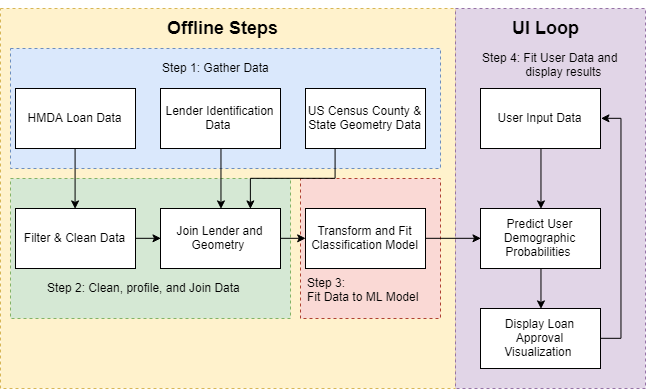
\includegraphics[width=\linewidth]{SparkDesignDiagram.png}

\end{frame}

\end{document}
